\fancychapter{User studies}
\label{chapter:results}

In order to evaluate the created social robot on the game playing scenario of \emph{Sueca}, a user study was conducted.
The main idea was to set up the environment in which this robot is supposed to interact with human players, and collect, in an adequate way, their feelings and perceptions.

The first measure this study aims to evaluate is trust, since \emph{Sueca} contains companionship between team players.
At the same time, this game includes two teams competing with each other and therefore, the influence of these conditions can also be calculated for every defined measure.
Additionally, measuring the social presence of every \emph{Sueca} partner will also provide a comparison between the two conditions.
Finally, the last chosen measure is affect in order to evaluate the evolution of participants' feelings.

%The targeting measures are the trust on the partner, the affect felt, and also the perception of the team player's social presence.
Participants answered two questionnaires, one before playing with \ac{emys} and one after.
The current chapter starts with the samples description and proceeds with analyses of the three mentioned measures.

\section{Methodology and Procedures}
Each session lasted an hour and involves 3 participants playing with \ac{emys}.
Firstly, each subject selected his team player in a draw.
Secondly, according to each condition, having a human or robot partner, participants answered a questionnaire before playing \emph{Sueca}.
This questionnaire, available in Appendix~\ref{appendixB} the robot partner version, contained two parts: the PANAS Questionnaire \cite{Egloff1998} and Human-Robot Trust Questionnaire \cite{Schaefer2013}.
Then, one researcher explained the game rules with a standard deck, and played some tricks until everyone felt comfortable.
After reviewing the \emph{Sueca} game, participants moved to the touch table and started a session of 5 games with or against \ac{emys}, considering the results in the initial draw.

\begin{figure}[h!]
  \centering
    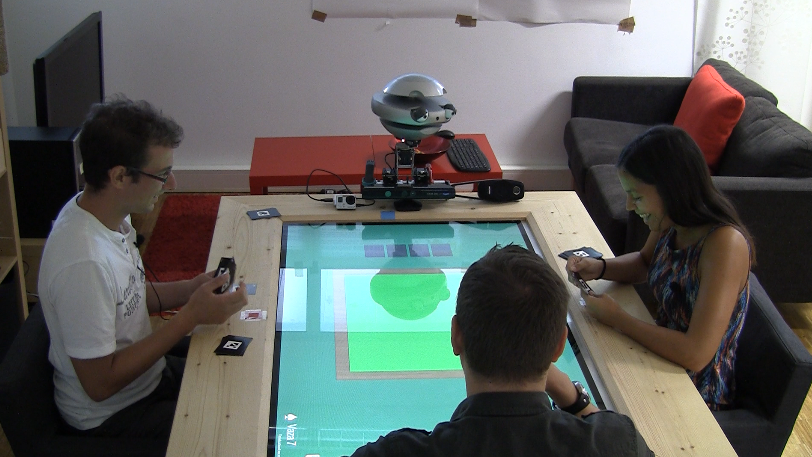
\includegraphics[width=0.8\textwidth]{./img/7/userStudies}
  \caption{Example of a game session}
\label{fig:userStudies}
\end{figure}

Lastly, participants answered another questionnaire, available in Appendix~\ref{appendixB} the human partner version, divided into four parts: the PANAS Questionnaire, Human-Robot Trust Questionnaire, the Networked Minds Questionnaire \cite{Harms2004} and some demographic questions.
All statistical analyses further mentioned used a significance level of 5\%.

\section{Samples Description}
\label{sec:samples}
A group of 60 participants were included in this study with a mean age of 24,31 $\pm$ 3,852.
Out of the 60 subjects, 40 played the game with a human partner and 20 played with \ac{emys}.
These distributions aimed to collect a valid number of answers from \ac{emys}' partners.
Additionally, out of the 59 subjects that revealed their gender, 20 were females and 39 were males.
Furthermore, most participants affirmed to know their partners in spite of not having played with them before, and their \emph{Sueca} knowledge was nearly medium.

\section{Trust}
\label{sec:trust}
The trust in the partner was measured by the answers of each individual to the Human-Robot Trust Questionnaire, before and after the game session.
Consequently, the following three study hypothesis arose:
\begin{itemize}
\item Are there changes in trust after the experience of interacting with the \emph{Sueca} partner?
\item Are the trust levels influenced by the partner (robot or human)?
\item Are the trust levels influenced by the game results?
\end{itemize}


\subsection*{Are there changes in trust after the experience of interacting with the \emph{Sueca} partner?}
The statistical test Mixed ANOVA was used to infer a conclusion about this question, with \emph{time} as a factor of 2 levels and \emph{condition} (partner) as the between-subjects factor.
Additionally, assumptions were tested to guarantee the results validity.
The dependent variable (\emph{time}) showed a significant effect with p = 0.03.
However, by adding the independent variable (\emph{condition}), the effect was not significant with p = 0.65.

\begin{figure}[h!]
  \centering
    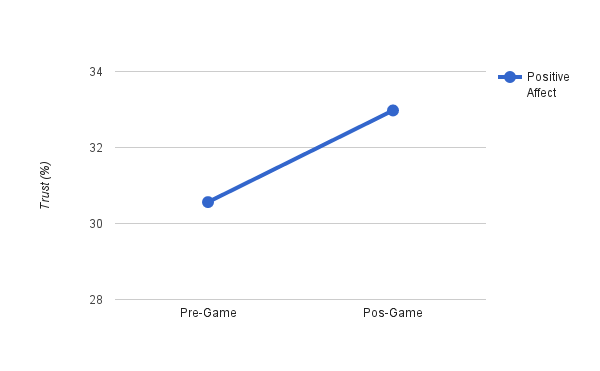
\includegraphics[width=0.7\textwidth]{./img/7/trustTime}
  \caption{Evolution of the trust percentage between the two time levels}
\label{fig:trustTime}
\end{figure}

Figure~\ref{fig:trustTime} presents the evolution of the trust percentage between the two time levels, before and after the game.
The trust values correspond to estimated means separated by time, since it was the only significant variable.

\textbf{Answer:} There were significant differences in Trust before and after playing \emph{Sueca}.
However, there was no significant differences in Trust before and after playing \emph{Sueca} for different partners.
Additionally, the trust levels of participants increased after playing \emph{Sueca} with \ac{emys}.



\subsection*{Are the trust levels influenced by the partner (robot or human)?}
The statistical test Welch Test was used to infer a conclusion about this question, with \emph{condition} as factor and \emph{final trust} as dependent variable.
As a result, the \emph{condition} effect was proved with p = 0, suggesting the means of trust were significantly different between having a robot partner or a human partner.

\begin{figure}[h!]
  \centering
    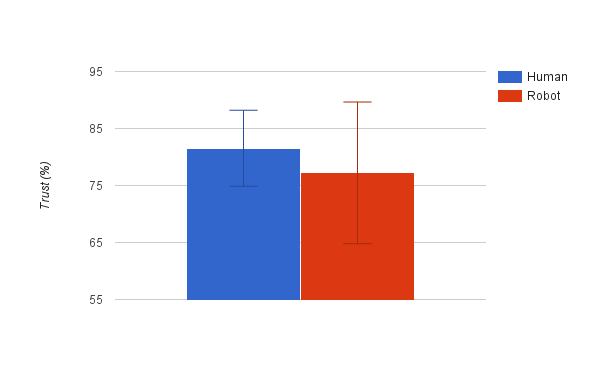
\includegraphics[width=0.7\textwidth]{./img/7/trustCondition}
  \caption{Differences of trust levels between conditions}
\label{fig:trustCondition}
\end{figure}

Figure~\ref{fig:trustCondition} evidences the trust level was higher for the \emph{condition} human partner, with a trust mean value of 81.538\%, when compared with the \emph{condition} robot partner, with a trust mean value of 77.215\%.

\textbf{Answer:} There were significant differences in Trust between different \emph{Sueca} partners.
Additionally, subjects' trust levels for human partners was higher than robot partners.


\subsection*{Are the trust levels influenced by the game results?}
A two-way ANOVA was run on data to analyse if the game results influenced the trust levels, with \emph{condition} and \emph{game result} as factors, and \emph{final trust} as dependent variable.
The effect of \emph{condition} was significant, with p = 0.01 (already proved in the previous question).
On the other hand, the \emph{game result} cannot reject the null hypothesis with p = 0.065, and therefore indicates a non significant effect on the trust measure.
Moreover, the effect of both \emph{condition} and \emph{game result} also proved to be non significant with p = 0.507.

\textbf{Answer:} There were no significant differences in Trust between different game results, which seems to suggest that independently of losing or winning the game, the perception of Trust in the game partner remains stable.


\section{Social Presence}
\label{sec:socialPresence}
After playing the game, each subject answered the Networked Minds Questionnaire in order to measure the social presence of his partner.
This measure of social presence includes six different subdimensions: co-presence, attentional allocation, perceived message understanding, perceived affective understanding, perceived emotional interdependence, and perceived behavioural interdependence.

By considering this measure in a \emph{Sueca} scenario, one study hypothesis arose:
\begin{itemize}
\item Is the social presence influenced by the partner (robot or human)?
\end{itemize}

\subsection*{Is the social presence influenced by the partner (robot or human)?}
The statistical test One-Way ANOVA was used to infer a conclusion about this question, with \emph{condition} as factor and each social presence subcategories' values as dependent variables.
\emph{Condition} presented the following statistical effects on each subdimension results:
\begin{itemize}
\item There was not a statistically significant difference between the \emph{co-presence} as determined by one-way ANOVA (F = 1.559, p = 0.217);
\item There was not a statistically significant difference between the \emph{attentional allocation} as determined by one-way ANOVA (F = 0.002, p = 0.965);
\item There was not a statistically significant difference between the \emph{perceived message understanding} as determined by one-way ANOVA (F = 0.081, p = 0.777);
\item There was a statistically significant difference between the \emph{perceived affective understanding} as determined by one-way ANOVA (F = 7.850, p = 0.007);
\item There was a statistically significant difference between the \emph{perceived emotional interdependence} as determined by one-way ANOVA (F = 4.148, p = 0.046);
\item There was not a statistically significant difference between the \emph{perceived behavioural interdependence} as determined by one-way ANOVA (F = 0.699, p = 0.406).
\end{itemize}

The social presence of partner evidenced discrepancies for the two conditions in two subdimensions: \emph{perceived affective understanding} and \emph{perceived emotional interdependence}.
As a result, Figure~\ref{fig:perceiveEmoAff} shows theses discrepancies, demonstrating the \emph{perceived affective understanding} and \emph{perceived emotional interdependence} were higher in human partners.

\begin{figure}[H]
  \centering
    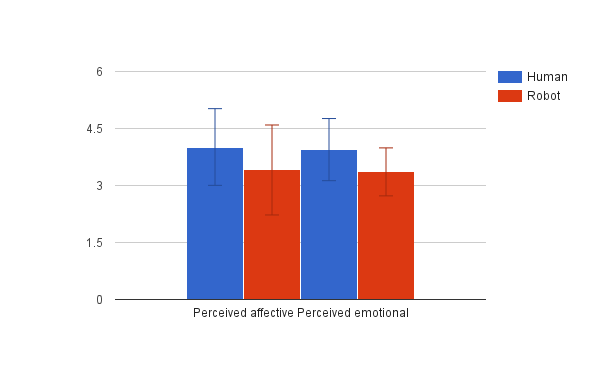
\includegraphics[width=0.7\textwidth]{./img/7/perceiveEmoAff}
  \caption{Perceived affective understanding and perceived emotional interdependence means for each  condition}
\label{fig:perceiveEmoAff}
\end{figure}

\textbf{Answer:} There were significant differences in Social Presence between \emph{Sueca} partners for two dimensions: perceived affective understanding and perceived emotional interdependence.
The mean values of both subdimensions were higher for human partners.
Additionally, there were no significant differences in the remaining subdimensions of Social Presence between \emph{Sueca} partners.


\section{Affect}
\label{sec:affect}
The affect was measured by the answers of each individual, before and after the game session, to the PANAS Questionnaire.
It is divided into positive and negative affects and, therefore, there are two study hypothesis:
\begin{itemize}
\item Are there changes in the positive affect after the experience of interacting with the \emph{Sueca} partner?
\item Are there changes in the negative affect after the experience of interacting with the \emph{Sueca} partner?
\end{itemize}

\subsection*{Are there changes in the positive affect after the experience of interacting with the \emph{Sueca} partner?}
In order to answer this questions, a Mixed ANOVA was run on the collected data, with \emph{time} as a factor of 2 levels and \emph{condition} as the between-subjects factor.
So, \emph{time} proved to have a statistical significant effect on the positive affect, p = 0.008.
On the other hand, \emph{time} levels for each \emph{condition} did not present a significant effect on the positive affect, p = 0.488.

\begin{figure}[h!]
  \centering
    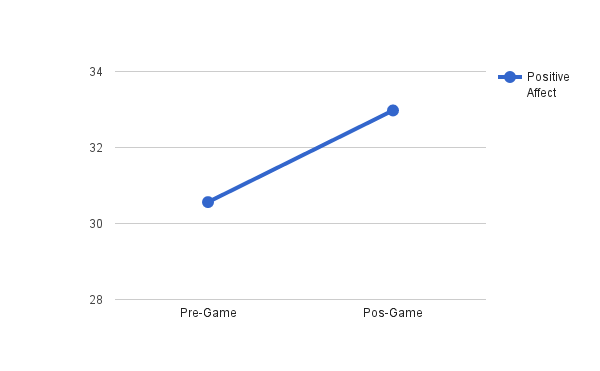
\includegraphics[width=0.7\textwidth]{./img/7/positiveAffect}
  \caption{Evolution of the positive affect between the two time levels}
\label{fig:positiveAffect}
\end{figure}

Figure~\ref{fig:positiveAffect} evidences the evolution of the positive affect before and after playing \emph{Sueca} with \ac{emys}.

\textbf{Answer:} There were significant differences in Positive Affect before and after playing \emph{Sueca}.
However, there were no significant differences in Positive Affect before and after playing \emph{Sueca} between different partners.

\subsection*{Are there changes in the negative affect after the experience of interacting with the \emph{Sueca} partner?}
In order to answer this questions, a Mixed ANOVA was run on the collected data, with \emph{time} as a factor of 2 levels and \emph{condition} as the between-subjects factor.
The dependent variable (\emph{time}) did not present a significant effect with p = 0.267.
Furthermore, by adding the independent variable (\emph{condition}) to \emph{time}, the effect was also not significant, with p = 0.184.

\textbf{Answer:} There were no significant differences in Negative Affect before and after playing \emph{Sueca}.
Also, there were no significant differences in Negative Affect before and after playing \emph{Sueca} influenced by different partners.

\section*{\centering*}

Overall, the difference on the trust levels between conditions suggested that humans cannot yet trust in robots, when playing \emph{Sueca}.
In addition, the trust levels were not influenced by the game result, which reinforces the importance of condition on this measure.
However, trust levels have increased after playing the game, without the influence of the condition.
On the other hand, the social presence of the partner, was not influenced by the condition in most subdimensions, suggesting this robotic \emph{Sueca} player was socially perceived as a human in those subdimensions.
The first difference influenced by the condition, on the \emph{perceived affective understanding}, suggests that people who had \ac{emys} as partner were either less able to perceive its affective state, or they found it difficult for \ac{emys} to understand their affective state.
The second difference influenced by the condition, on the \emph{perceived emotional interdependence}, suggests that people who had \ac{emys} as partner were either less affected by its affective state, or they found \ac{emys} was less affected by their affective state.
Interestingly, the second difference may be caused the first one.
Finally, even though the negative affect did not change after the game with \ac{emys}, the positive affect increased after the game, suggesting it was a pleasing experience for participants.


\cleardoublepage
